%
% teil1.tex -- Beispiel-File für das Paper
%
% (c) 2020 Prof Dr Andreas Müller, Hochschule Rapperswil
%
% !TEX root = ../../buch.tex
% !TEX encoding = UTF-8
%
\section{Modellbildung
\label{openfoam:section:teil1}}
\kopfrechts{Modellbildung}
Zum Simulieren von Strömungen benötigen wir zum einen ein Modell, das das Verhalten des Mediums, im Fall einer Strömungssimulation eine Flüssigkeit, möglichst umfassend und genau beschreibt. 
Hierbei werden meist die Navier-Stokes Gleichungen benutzt, welche noch mit der Kontinuitätsgleichung und Energiegleichung erweitert jedoch werden auch in einigen Fällen die Euler-Gleichungen oder die Potentialgleichungen verwendet, da diese zwar ein weniger vollständiges Modell beschreiben, jedoch weniger Rechenintensiv sind.

Zudem benötigen wir ein Lösungsverfahren, das einen Anfangszustand und das mathematische Modell zu einer Numerischen Lösung verarbeiten kann, dies ist nötig da für die Navier-Stokes-Gleichungen keine analytische Lösung existiert und die der Euler-Gleichungen sehr aufwendig sind zu berechnen. 
Hierbei kommen meist die Finite-Differenzen-Methode (FDM), die Finite-Volumen-Methode (FVM) und die Finite-Elemente-Methode (FEM) zum Einsatz. 

OpenFOAM nutzt dabei in den meisten Fällen die FVM. 
Dabei ist jedoch auch zu erwähnen, dass OpenFOAM sich besonders dafür eignet, neue algorithmische Lösungsverfahren zu implementieren und zu testen.

\subsection{Stationär oder Zeitabhängig?}
Bei der Strömungsmechanik wird zuerst unterschieden, ob es sich um eine stationäre oder zeitabhängige Strömung handelt.
Das heisst es ist entweder der Fall, dass an jedem Ort im Raum die Geschwindigkeit, der sich dort befindenden Flüssigkeit in Bezug auf Betrag und Richtung konstant ist (stationär) oder dass sich diese Grösse ändert (zeitabhängig).
Bei einer Simulation wird meist simuliert bis der stationäre Zustand, bis auf einen kleinen Fehler, erreicht wird.
Dadurch kann man sich Simulationsaufwand ersparen da sobald der stationäre Zustand erreicht wird das Resultat nicht mehr ändert und so keine neuen Ergebnisse gefunden werden können.

\subsection{Modellierung der Flüssigkeit}
Im Kontext der CFD-Simulation nimmt man an, dass eine Flüssigkeit nicht aus einzelnen Teilen wie Atomen oder Molekülen besteht, sondern man nimmt an, dass die Flüssigkeit kontinuierlich, also ohne Zwischenräume, ist. 
Zudem wird angenommen, dass sämtliche Eigenschaften, die sich von Punkt zu Punkt innerhalb der Flüssigkeit Stetig und die Ableitung davon ebenfalls stetig sind. 

Zudem hat eine Flüssigkeit noch weitere Eigenschaften wie die Dichte. 
Diese kann hier aber nicht immer als konstant angesehen werden, da man ansonsten bei kompressiblen Flüssigkeiten einen Teil der Energie, welcher für das Komprimieren dieser verwendet wird, nicht beachten würde.
%TODO REYYNOLDS
Dies wiederum würde im Fall, dass die Kompressibilität beachtet werden muss zu Abweichungen zwischen Simulation und Realität führen, da die Simulation die Gesetze der Energie und Massenerhaltung nutzt um die 
Zudem müssen die Viskosität und die spezifische Wärmekapazität, wobei die Viskosität in der Navier-Stokes-Gleichung benötigt wird, beschrieben werden.

\subsection{Die Euler-Gleichungen}
Die Euler-Gleichungen beschreiben das Verhalten der Strömung eines reibungsfreien Fluiden, also eines Laminaren Flusses dessen Reibung vernachlässigt werden kann. 
Das bedeutet sie können nicht für alle Probleme eingesetzt werden da sobald Reibungskräfte einen substantiellen Einfluss auf die Strömung haben, das Berechnete Ergebnis eine zu grosse Abweichung aufweist.

\subsubsection{Massenerhaltung}
Das Gesetz der Massenerhaltung beschreibt, dass in einem geschlossenen System sich die Masse nicht verändert, ohne dass man Masse hinzufügt oder entfernt. 
Dieses Verhalten beschreibt die zweite Euler-Gleichung, indem die Veränderung der Masse durch den Fluss von Masse durch eine Systemgrenze beschrieben wird.

Die Erste Euler Gleichung geht aus der Idee hervor, dass man ein beliebiges Volumen $V$ hat, das fest im Raum liegt. Durch ein Oberflächenstück 
$d \vb{S} $ 
des Volumens 
$V$
 fliesst jeweils der Massenstrom 
$\vb{S} \cdot\rho\vb{u}$.
Aus dem Massenstrom des Oberflächensegments kann man dann mit dem Oberflächenintegral 
\[\int_{S}d\vb{S}\cdot\rho\vb{u}\]
den Gesamten Massenstrom berechnen. Dieser Massenstrom muss nun gleich sein wie die Massenänderung der in dem Volumen enthaltenen Flüssigkeit 
\[\frac{\partial M}{\partial t}\]
dies lässt sich mit dem Integral 
\[\int_{V}\frac{\partial \rho}{\partial t} dV\]
berechnen, hier integriert man die Dichteänderung in einem Volumenelement über das ganze Volumen 
$V$ 

Setzt man nun die beiden Terme gleich erhält man die Gleichung 
\[\int_{S}d\vb{S}\cdot\rho\vb{u} 
=
\int_{V}\frac{\partial \rho}{\partial t} \, dV ,\] 
bei dieser Gleichung kann man nun auf der L.H.S. mit dem Gaussschen Integralsatz das Oberflächen Integral in ein Flächenintegral umwandeln es wird also zu
\[\int_{V}\nabla\cdot(\rho\vb{u}) 
=
\int_{V}\frac{\partial \rho}{\partial t} \, dV \]
mit dem Ändern der Flussrichtung und umschreiben der Gleichung kann man die R.H.S auf null setzen und die Integrale zu einem Integral
\[\int_{V}\frac{\partial \rho}{\partial t} + \nabla\cdot(\rho\vb{u})  \, dV 
= 
0\]
zusammenfassen.

Dies kann nun in einem letzten Schritt in die Differentialgleichung
\begin{equation}
\label{openfoam:euler1}
\frac{\partial \rho}{\partial t} + \nabla\cdot(\rho\vb{u})  \, dV 
= 
0
\end{equation}
umwandeln.

\subsubsection{Impulserhaltung}
Die zweite Euler Gleichung beschreibt das Gesetz der Impulserhaltung, es besagt dass der Gesamtimpuls eines mechanisch abgeschlossenen Systems konstant ist.
Dies wird beschrieben, indem die Änderung des Impulses eines Systems aus der aussen am System Anliegenden Kraft und Kräfte, die auf das System wirken wie die Schwerkraft.

Bei der Impulserhaltung geht man fast gleich vor wie beim Herleiten der Gleichung für die Massenerhaltung.
Man geht ebenfalls von einem beliebigen Volumen Flüssigkeit, $V$, das nicht mehr fest an Ort und beliebigem Masseninhalt ist, sondern eine feste Menge Masse, die sich durch den Raum bewegt.
Dieses Volumen weist nun eine Impulsänderung die
\[\frac{D}{Dt}\int_{V}\rho\vb{u}\, dV\]
entspricht.

Als nächstes berechnet man die gesamte kraft auf die Oberfläche des Volumens $V$ in dem man alle Kräfte $\vb{f} = \vb{t}\,dS$, die auf die Oberflächenstücke $dS$ wirken, integriert.
Wobei $\vb{t} dS$ gleich $(\vb{n\cdot\sigma}dS)$ ist. 
Daraus erhält man die Kraft 
\[\vb{Fs} 
=
\int_{S}\vb{f}\, dS
= \int_{S} (d\vb{S}\cdot\vb{\sigma})
\]
Dies ist nun wieder ein Flächenintegral, das mit dem Gaussschen Integralsatz in ein Volumenintegral umgewandelt werden kann.
Dadurch ergibt sich, dass
\[\vb{Fs} 
=
\int_{V}\nabla \cdot \vb{\sigma}\, dV
.\]

Zuletzt berechnen wir noch den Einfluss anderer Kräfte wie die Schwerkraft auf den Impuls des Volumens $V$.
Dazu integrieren wir den Vektor $\vb{b}$, bei dem es sich um eine Beschleunigung handelt, über alle Volumenstücke $dV$ wodurch wir das Integral
\[\vb{Fa} 
=
\int_{V}\rho\vb{b}, dV
\]
erhalten.

Nun können wir die Impulsänderung des Volumens gleich der Summe der darauf wirkenden Kräfte setzen und die Integrale in einem Integral zusammenfassen, daraus erhalten wir, mit der Bedingung die Masse im Volumen sei konstant, die Gleichung 
\[\int_{V} \rho \frac{D\vb{u}}{Dt} - \nabla \cdot \vb{\sigma} -\rho \vb{b}\, dV
=
0
\]
hierbei kann man das Integral wieder weglassen wodurch wir die Differentialgleichung
\begin{equation}
\label{openfoam:euler2_1}
\rho \frac{D\vb{u}}{Dt}
= 
\nabla \cdot \vb{\sigma} +\rho \vb{b}
\end{equation}
erhalten.

Zuletzt kann man noch die substantielle Ableitung in eine partielle umwandeln damit wir die gleiche Form wie für die Massenerhaltungs Gleichung erhalten.
Dazu nutzen wir die Definition der substantiellen Ableitung
\[
\frac{D\Phi(\vb{x},t)}{Dt}
:=
\frac{\partial \Phi}{\partial t}+(\vb{u}\cdot \nabla)\Phi
\] 
eingesetzt in die Differentialgleichung erhalten wir so 
\begin{equation}
\label{openfoam:euler2}
\rho\frac{\partial\vb{u}}{\partial t} + \nabla \cdot(\rho\vb{u}\vb{u})
= 
\nabla \cdot \vb{\sigma} +\rho \vb{b}.
\end{equation}
Diese Form erleichtert einem die Berechnung, da sie nicht mehr die Impulsänderung einer sich bewegenden Menge Flüssigkeit beschreibt, sondern die Impulsänderung der sich momentan an einem Ort befindenden Masse. Man kann also anstelle ein sich durch den Raum bewegendes Masseteilchen ein Festes Volumenelement Simulieren, welches bei der Fluiddynamik-Simulation die bevorzugte Methode ist.

\subsubsection{Energieerhaltung}
Die dritte der Euler-Gleichungen wurde nicht wie die der Masse- und Impulserhaltung von Leonhard Euler hergeleitet, sie wird jedoch auch als Euler-Gleichung bezeichnet.

Das Gesetz der Energieerhaltung besagt, dass die gesamte Energie in einem isolierten System konstant bleibt.
Diese Energie setzt sich im Fall der Fluiddynamik aus kinetischer, potenzieller und thermischer Energie zusammen.
Sie wird verändert durch mechanische Arbeit, die äussere Kräfte leisten. Ebenso können Wärmequellen den Wärmeinhalt beeinflussen.

Die dritte Euler-Gleichung beschreibt dieses Naturgesetz mit der Differentialgleichung 
\begin{equation}
\label{openfoam:euler3}
\rho \frac{De}{Dt}+  \rho \frac{DK}{Dt}
=
- \nabla \cdot \vb{q} + \rho r + \nabla \cdot (\sigma \cdot \vb{u}) + \rho \vb{b} \cdot \vb{u} 
,\end{equation}
welche besagt dass die Änderung der thermischen Energie $\rho \frac{De}{Dt}$ und die der kinetischen $\rho \frac{DK}{Dt}$ (wobei $\rho K$ die kinetische Energie $\rho \frac{\abs{\vb{u}}^{2}}{2}$ ist) zusammen die gesamte Änderung der Energie im Volumenelement $V$ sind.
Diese gesamte Energieänderung wird aus dem Zufluss mechanischer und thermischer Energie, aber auch durch Hitze und mechanische Leistungsquellen im Inneren des Volumens, berechnet.
So ist der Zufluss, ins Innere des Volumen, aus den Termen $- \nabla \cdot \vb{q}$ und $\nabla \cdot (\sigma \cdot \vb{u})$ welche den Zufluss thermischer respektive mechanischer Energie durch die Oberfläche des Volumens darstellen.
Dazu kommt noch die Änderung der Energie durch Quellen im Inneren des Volumens durch Hitzequellen $\rho r$ und Mechanische Energiequellen $\rho \vb{b} \cdot \vb{u}$.

\subsection{Navier-Stokes}
Die Navier-Stokes Gleichungen sind eine Erweiterung der Euler-Gleichungen, welche zusätzlich noch die Viskosität der Flüssigkeit berücksichtigen.
Dadurch können Flüssigkeiten genauer modelliert werden als mit den Euler-Gleichungen, da in Fällen in denen die Reibung der Flüssigkeit einen grossen Einfluss auf das Resultat hat, das Modell vollständiger ist.

Dabei ist die Erste Gleichung, die wir benötigen die Massenerhaltungs-Gleichung 
\[\nabla \cdot \vb{u}
=
0
,
\]
die wir schon, in einer etwas umfassenderen Form, in Gleichung \eqref{openfoam:euler1} beschrieben haben.
Dazu benötigen wir noch die Navier-Stokes Impulserhaltungs-Gleichung 
\begin{equation}
\rho \frac{D\vb{u}}{Dt}
=
- \nabla p + \mu \delta \vb{u} +\rho \vb{b} 
,\end{equation}
in dieser werden mit den Termen $- \nabla p$ und $\mu \delta \vb{u}$ interne Kräfte und mit dem Term $\rho \vb{b}$ externe Kräfte, wie zum Beispiel Schwerkraft oder eine Elektrostatische Kraft (gleich wie in Formel \eqref{openfoam:euler2}), ausgedrückt.
Der Term $- \nabla p$ beschreibt die Kräfte, die durch einen Druckunterschied zwischen verschiedenen Orten entstehen.
Hier wird also die durch einen Druckunterschied hervorgehenden Kraft zur Ganzen Impulsänderung dazugerechnet.
Der letzte verbleibende Term $\mu \delta \vb{u}$ beschreibt die internen Reibungskräfte.
Dabei beschreibt $\mu$ die kinematische Viskosität der Flüssigkeit, welches die Proportionalitätskonstante die beschreibt wie viel Kraft benötigt wird um zwei Schichten der Flüssigkeit mit unterschiedlicher Geschwindigkeit aneinander vorbei zu bewegen ist.
Zuletzt wird mit dem Term $\mu \delta \vb{u}$ ein diffusiver Impulstransport beschrieben, also wie durch die Reibungskräfte zwischen Teilchen mit unterschiedlicher Geschwindigkeit ein Impulsstrom zwischen ihnen, auf Grund der Viskosität stattfindet.

Zusammen beschreiben die beiden Gleichungen eine inkompressible Flüssigkeit spannend ist hier noch, dass die Gleichung, die die Energieerhaltung beschreibt, nicht mehr benötigt wird. 

\subsection{Objekt Modellierung}
Bei der CFD Simulation müssen nicht nur die Physikalischen Eigenschaften des Mediums, sondern auch die Form des Objektes dessen Influenz auf die Flüssigkeit und die Umgebung in der sich das Objekt befindet simuliert werden soll Modelliert werden.
Dazu gehören zum einen die Geometrischen Eigenschaften des Objektes und die Umgebung in dem es sich befindet, zudem aber auch die Eigenschaften wie die Oberflächen der Objekte mit der Flüssigkeit interagieren.

Zum Modellieren der Objekte kann man eine beliebige CAD Software benutzen, für OpenFOAM muss dieses Modell dann jedoch konvertiert werden.
Dazu ist eine Software, snappy hex  mesh, die bei OpenFOAM beinhaltet ist verfügbar.
Sie verarbeitet das 3D Modell, meist im STL Format, zusammen mit einem simpleren Modell für die Begrenzung der Lösungs-Domain, welches für OpenFOAM bei simplen Geometrien am beste im blockMesh Format definiert wird, zusammen um zum einen die Form der Lösungs-Domain (Raum in der sich die Flüssigkeit in der Simulation befindet) zu generieren und zudem eine Diskretisierung der Flächen und Unterteilung des Raumes in Zellen.
Diese Diskretisierung ist benötigt, dass die Finite Volume Methode verwendet werden kann um das Mathematische Modell der Flüssigkeit auf der Lösungs Domain anzuwenden.
Ein Beispiel dafür ist in Bild \ref{openfoam:fig:SD_Modell_vergleich} zu sehen.
\begin{figure}[h]
	\centering
	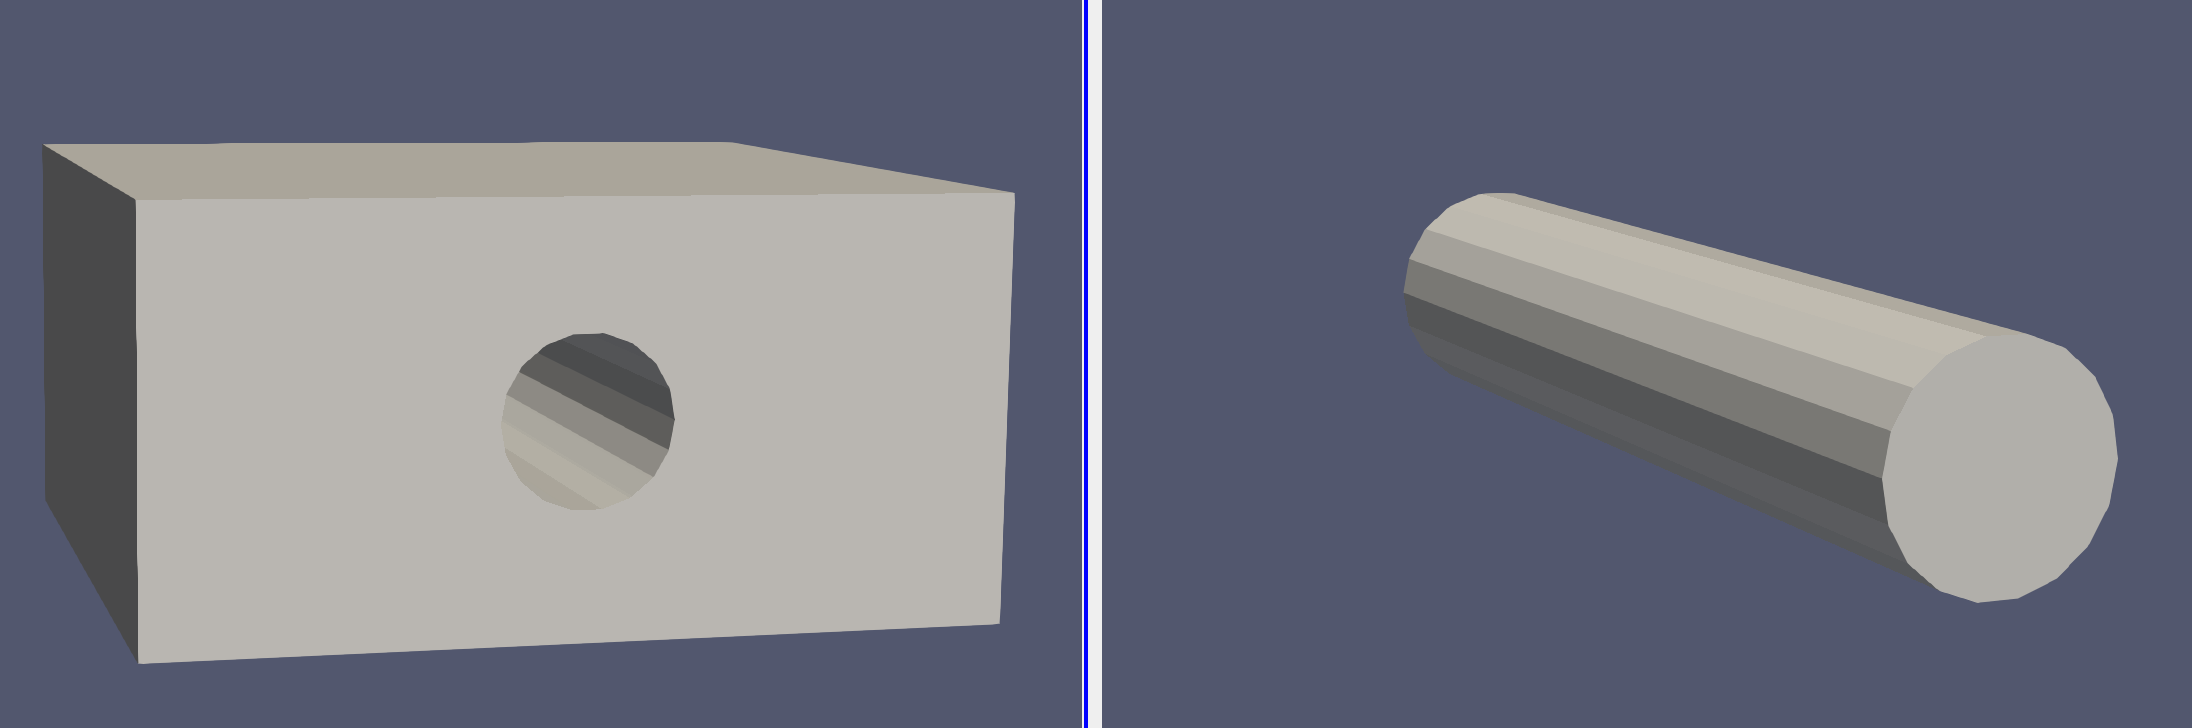
\includegraphics[scale=0.1]{papers/openfoam/Bilder/vergleich_solution_domain_object.png}
	\caption{Vergleich der Solution Domain (L) und dem 3D Modell des Objektes (R)}
	\label{openfoam:fig:SD_Modell_vergleich}
\end{figure}

In Bild \ref{openfoam:fig:sim_grid} ist zudem ein Beispiel für die Unterteilung der Geometrie in Zellen zu sehen.
Darauf sieht man einen weiteren Vorteil des Gitters, es wird nahe dem Objekt nämlich die Grösse der Zellen verringert.
Dadurch kann der Rechenaufwand, der ansonsten betrieben werden muss, um die ganze Lösungsdomain mit dem feineren Gitter zu lösen, das wir für genügend Detail am Objekt benötigen, verringert werden.

\begin{figure}[h]
	\centering
	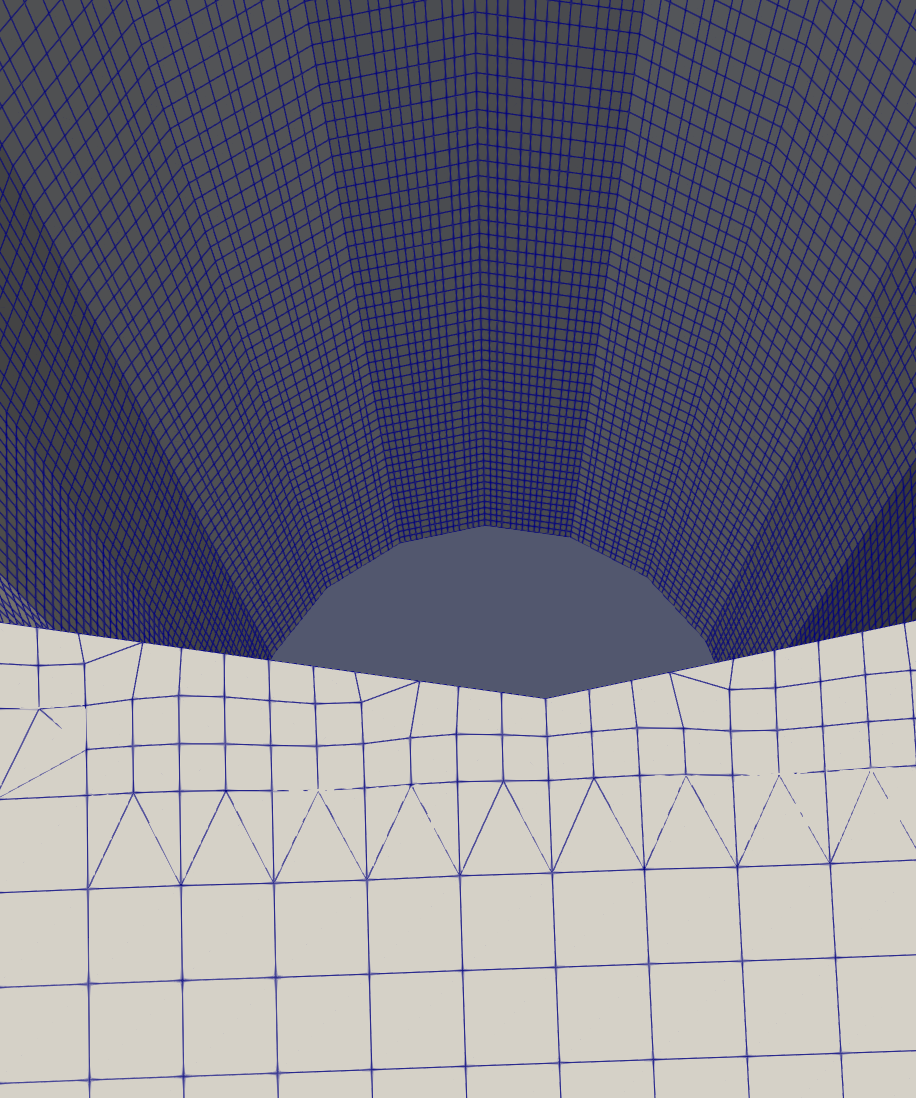
\includegraphics[scale=0.1]{papers/openfoam/Bilder/grid.png }
	\caption{Beispiel des Rechengitters das von Snappy Hex Mesh generiert wird}
	\label{openfoam:fig:sim_grid}
\end{figure}
Zudem ist auch zu sehen, dass die Zellen nicht unbedingt Würfel sein müssen das Netz kann theoretisch aus beliebigen Polyedern bestehen, dies ist aber nicht unbedingt vorteilhaft, denn es ist anzustreben ein Seitenverhältnis der Zellen von ungefähr eins zu wählen dies spart Zeit beim Verarbeiten der 3D Modellen zum Mesh.

\subsection{Boundary Conditions}
Mit den Boundary Conditions definiert man wie die Flüssigkeit mit einer Zellenwand interagiert.
Dabei ist aber zu sagen, dass dies nicht nur Physikalische Oberflächen sondern auch Symmetrieachsen, Inlet und Outlet Zellen, Thermische Elemente und viele mehr darstellen können.

\subsubsection{Inlet}
Im Falle eines Inlets wird ein Fester Wert an der Oberfläche des Patches festgelegt. So werden zum Beispiel die Geschwindigkeit und Temperatur über eine Fläche fest bestimmt, dabei ist jedoch wichtig zu beachten das der Druck und die Geschwindigkeit nicht unabhängig voneinander sind, dadurch muss der Druck frei belassen werden und es wird anstelle eines Festen Wertes der Gradient des Druckes fest auf null gesetzt. 
Dadurch kann auch eine Variable Eingangsgeschwindigkeit bestimmt werden, dies ist zum Beispiel nützlich, wen man den Blutfluss durch eine Arterie Simulieren will, da man mit einer sich zyklisch ändernder Geschwindigkeit den vom Herz aus pulsierenden Fluss modellieren kann.

\subsubsection{Outlet}
Ein Outlet wird meist genau umgekehrt modelliert als der Inlet dabei wird die Temperatur und Geschwindigkeit nicht auf einen festen Wert gelegt, sondern der Gradient dieser Variablen auf null gesetzt und der Druck wird auf einen festen Wert gelegt, jeweils auf den Umgebungsdruck, der ausserhalb der Simulierten Region herrschen soll.

\subsubsection{Wände}
Zudem benötigen wir jeweils noch Bedingungen wie die Flüssigkeit mit dem Objekt selbst und mit den Grenzen der simulierten Region interagiert.
Dazu nutzt man im Falle einer undurchlässigen Wand die sogenannte No-Slip Bedingung, diese setzt die Geschwindigkeit der Flüssigkeit an der Wand in normaler Richtung auf null und die tangential zur Wand auf dieselbe Geschwindigkeit dieser, welche meist auch null ist. 
Dadurch kann die Grenzschicht modelliert werden, da diese besagt, dass die Luft, die an einer Oberfläche entlang fliesst, in der Nähe der Fläche die Gleiche Geschwindigkeit dieser Oberfläche hat.
Dabei ist die Dicke dieser unbewegten Luftschicht abhängig von der Luftgeschwindigkeit und der kinematischen Viskosität.
Alternativ gibt es zu der No-Slip Bedingung noch weitere Modelle, um Undurchlässige Flächen zu modellieren.
So kann man zum Beispiel mit dem OpenFOAM Schlüsselwort \texttt{nutRoughWallFunction} eine raue Oberfläche modellieren, dabei müsste man jedoch noch weitere Parameter angeben, mit denen die Rauheit der Oberfläche spezifiziert wird.

Zusätzlich zu Boundary Conditions die das Physikalische Verhalten von Flüssigkeiten beschreiben gibt es noch solche die dazu genutzt werden können den Simulationsaufwand zu verringern.
Man kann damit Symmetrie Ebenen oder Achsen beschreiben, die in Fällen, in denen die Lösungs Domain Symmetrien aufweist, das Problem vereinfacht ohne Genauigkeit der Lösung einzubüssen.

\begin{figure}[h]
	\centering
	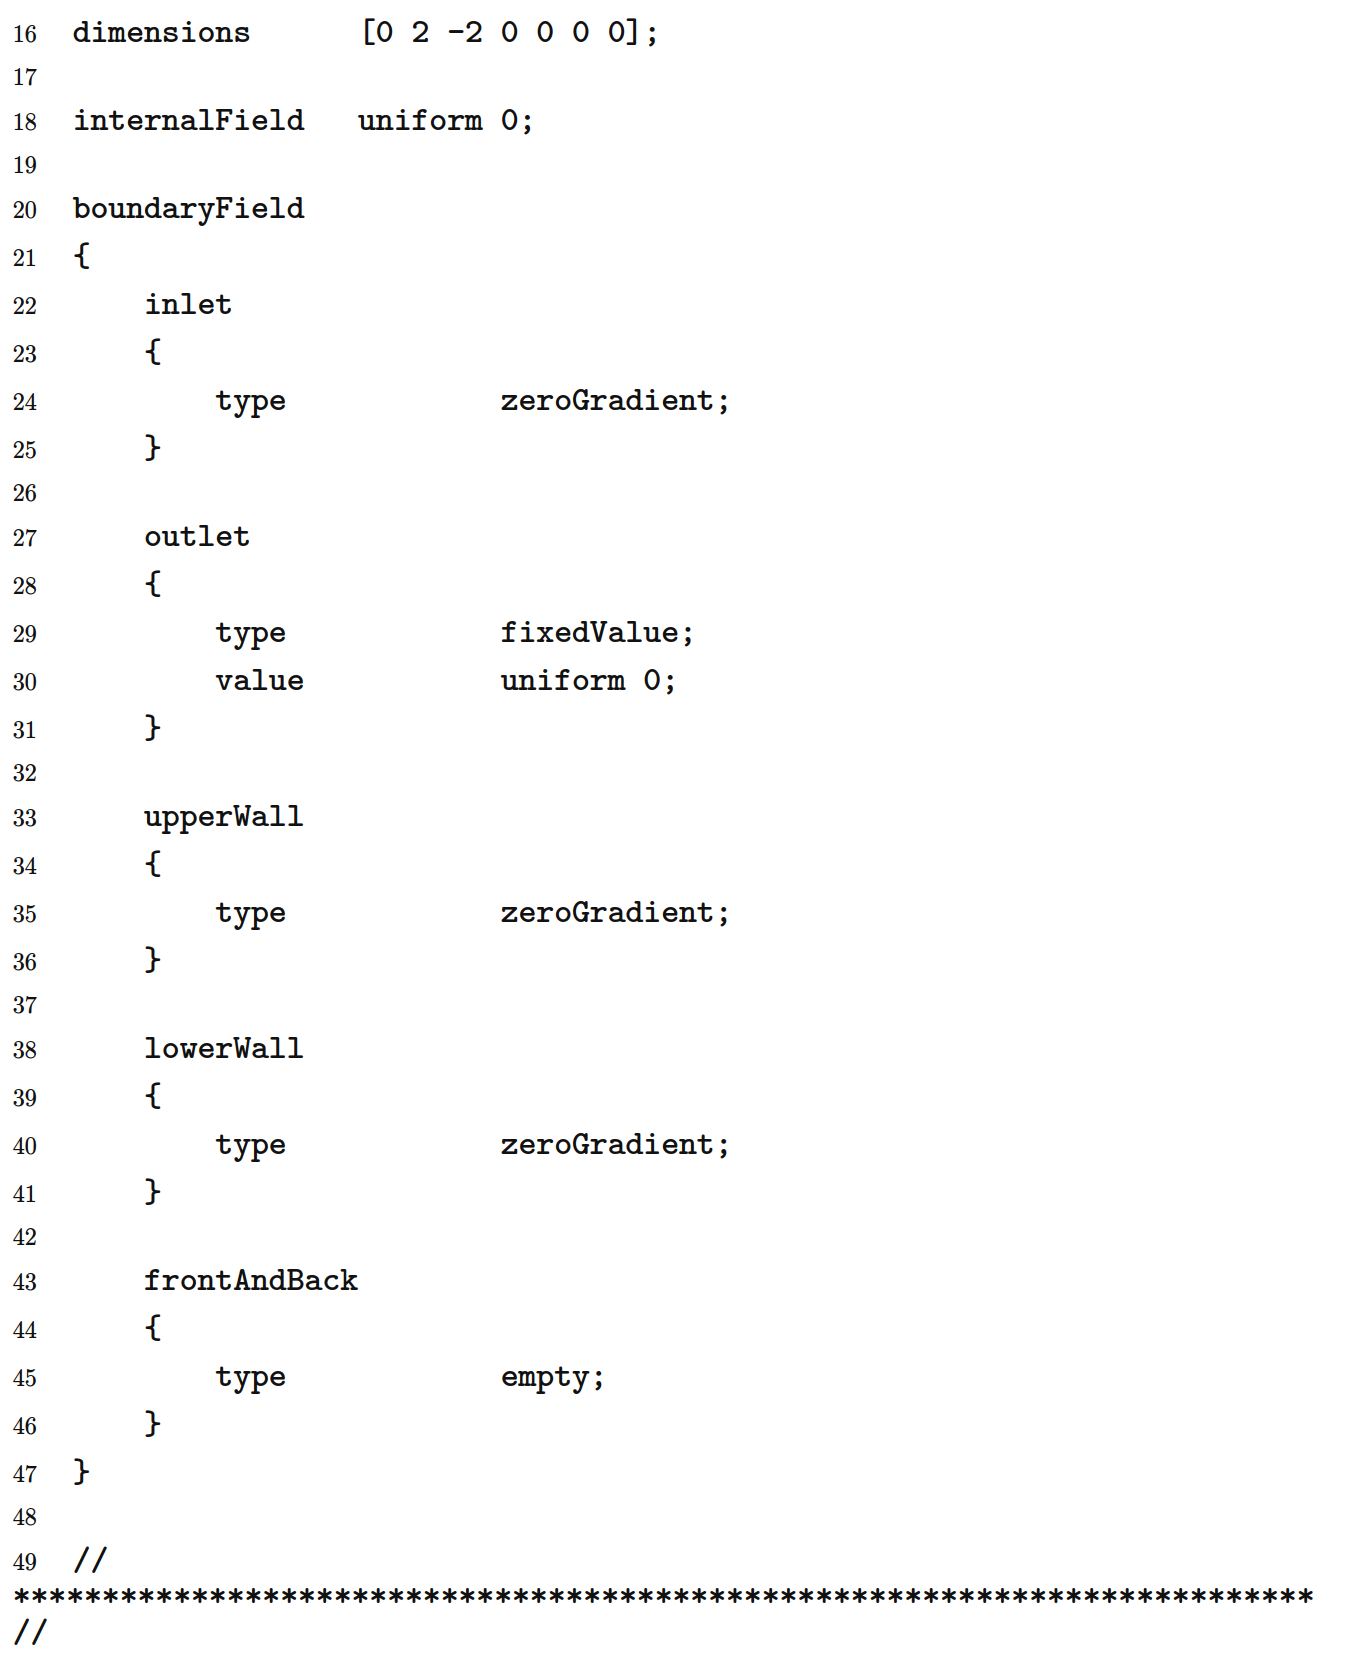
\includegraphics[scale=0.14]{papers/openfoam/Bilder/beispiel_boundarycond.png }
	\caption{Beispiel der Boundary Conditions in \texttt{0/p}(OpenFOAM v13 User Guide)}
	\label{openfoam:fig:boundarycond}
\end{figure}

Bei OpenFOAM werden die Eigenschaften der Patches in den Files \texttt{0/p} und \texttt{0/u} zusammen mit den initialen Bedingungen festgelegt. Davon ist ein Beispiel in Bild \ref{openfoam:fig:boundarycond} zu sehen.

\section{Software basiertes Lösen von Differentialgleichungen}
Wenn ein Modell für die Flüssigkeit, die Grenzbedingungen, das Objekt und dessen Umgebung vorhanden ist benötigt man nun ein Verfahren, um eine Lösung zu finden. 
Dazu muss die Software als erstes eine Diskretisierung der Differentialgleichungen die die Flüssigkeit beschreiben, durchführen.
Dabei wird das schon diskretisierte Netz der Lösungsdomain genutzt um die Komplexen Differentialgleichungen wie die der Navier-Stokes-Gleichungen in lineare Gleichungen für jede einzelne der Zellen umzuwandeln.
Um diese Linearisierung zu erreichen, werden jeweils die Eigenschaften der Flüssigkeit, wie Druck, Geschwindigkeit oder Temperatur, am Ort der Zellen durch die Werte in allen anderen Zellen berechnet.
Dabei wird der Wert in jeder Zelle, z.B. für Druck $p_N$ mit einem Koeffizienten $ a_{N} $ multipliziert und danach mit allen anderen addiert das Resultat davon ist jeweils ein weiterer Koeffizient $b_N$.
Dabei werden die Koeffizienten $a_{NN}$ und $b_{N }$ jeweils aus den Differentialgleichungen hergeleitet, die Methode dafür unterscheidet sich je nach welcher Methode (FDM, FVM oder FEM).
Dies führt dazu dass die meisten der Koeffizienten $a_{}$ null sind da die Werte einer Zelle nur von den Zellen die direkt an sie angrenzen abhängig sind.
Diese Summen kann man nun in Matrizen-Form bringen, dadurch erhält man für jede Eigenschaft eine Gleichung der Form
\begin{equation}
\begin{bmatrix}
	a_{1,1} &  a_{1,2} & a_{1,3} & \dots & a_{1,N} \\
	a_{2,1} &  a_{2,2} & a_{2,3} &  & a_{2,N} \\
	a_{3,1} &  a_{3,2} & a_{3,3} &  & a_{3,N} \\
	\vdots & &  & \ddots & \vdots \\
	a_{N,1} &  a_{N,2} & a_{N,3} & \dots & a_{N,N} \\
\end{bmatrix}
\begin{bmatrix}
	p_{1} \\
	p_{2} \\
	p_{3} \\
	\vdots \\
	p_{n}
\end{bmatrix}
= 
\begin{bmatrix}
b_{1} \\
b_{2} \\
b_{3} \\
\vdots \\
b_{n}
\end{bmatrix}
.
\end{equation}
Um nun den $p$ Vektor zu berechnen wird nicht die Gauss Methode verwendet, da dies für Matrizen der Grösse, die in CFD Simulationen entstehen, sondern es werden Iterative Methoden wie die Gauss-Seidel Methode verwendet.
Diese führen schon nach wenigen Iterationen zu einer recht genauen Lösung.